\cleartooddpage[\thispagestyle{empty}]
\chapter{Gamma Rays}

As this thesis searches for dark matter from the presence of gamma rays, a discussion on gamma rays and their properties is necessary.
These discussions revolve around three main topics: astrophysical mechanisms for creating gamma rays, gamma-ray-induced air showers in the Earth's atmosphere, and the different features of the Galactic Center relevant to gamma rays and this thesis.


\section{Methods of Creation}

There are three astrophysical mechanisms that are predicted to produce gamma rays at TeV energies.
The leptonic mechanism is when gamma rays' last energetic interaction is with electrons, while the hadronic mechanism is when gamma rays are created via proton interactions.
The third mechanism, one explored in this thesis, is when two WIMP dark matter particles annihilate either directly or indirectly into gamma rays.

In leptonic production, stars and galaxies have their own magnetic fields, and also emit electrons.
Inverse compton (\cite{compton_effect}) scattering can occur, where electrons and ambient photons collide, transferring energy to the photon.
After multiple repetitions of this, a small fraction of the original photon population can achieve TeV-scale energies.
Additionally, electrons spiralling through magnetic fields can produce synchrotron photons with X-Ray energies, meaning fewer inverse compton scatterings are needed to reach TeV energies \cite{self_compton}.
Other mechanisms can increase the number of TeV photons produced by a source, including stronger magnetic fields, breaking/reconnecting magnetic fields, as well as nearby ambient clouds of electrons.

In hadronic processes, protons are first accelerated by fermi acceleraton, emitted as part of a jet (\cite{hadronic1},\cite{hadronic2}), or another mechanisms.
Then, upon striking an ambient atom, the proton will decay into $\pi^{+}$, $\pi^{-}$, and $\pi^{0}$.
The $\pi^{0}$ then quickly (<1sec) decays into a $\gamma\gamma$ pair, with \nicetilde $\frac{1}{10}$th the original proton's energy.
Much of the diffuse gamma ray component of the galactic disk is believed to be due to extra-galactic high-energy protons colliding with the atoms of the dusty galactic plane. {\color{red}(cite??)}


\subsection{Dark Matter Interactions}
As discussed in various extensions of SUSY{\color{red}(cite??)}, dark matter may be detectable by three general detection schemes, illustrated in Figure \ref{fig:3_searches}.

% add popular figure for the three detection type
\begin{figure}[ht]
  \centering
  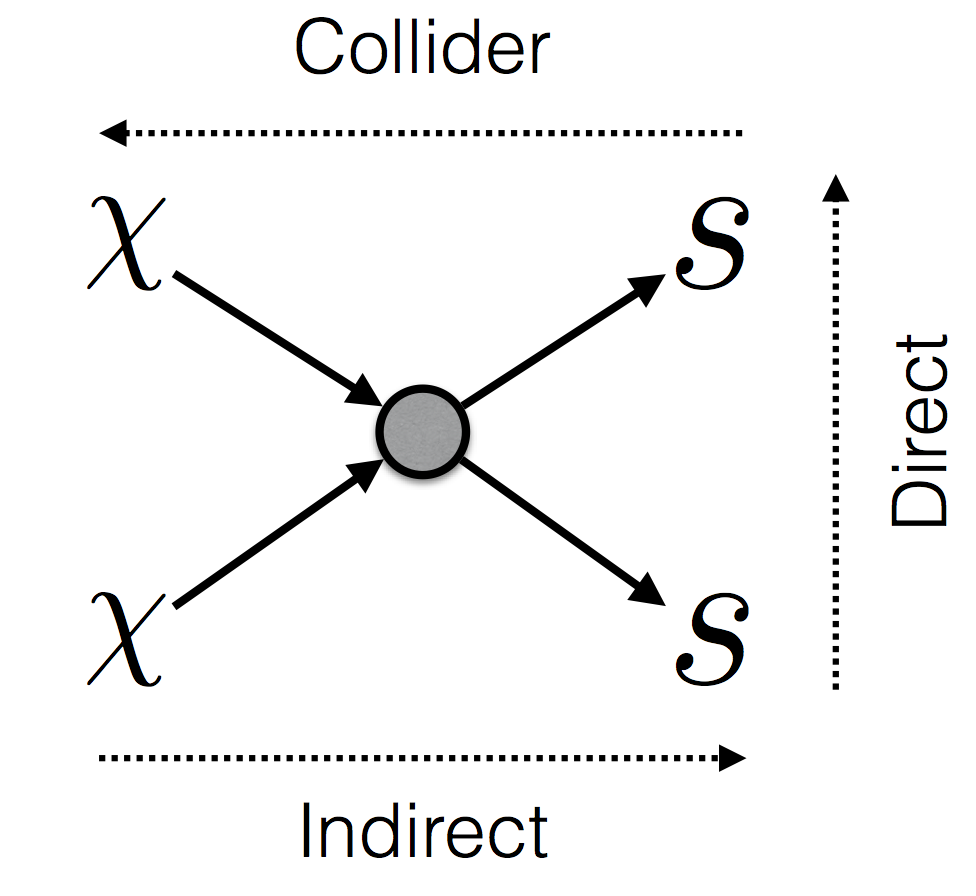
\includegraphics[width=0.45\textwidth]{images/3waystodetect.eps}
  \caption[3 Search Techniques]{
    The three general search techniques for dark matter.}
  \label{fig:3_searches}
\end{figure}

In Collider detection, $ss \rightarrow \chi\chi$, standar model particles ($ss$) are accelerated and collide in a detector, and the resulting particle fragments are measured by a slew of measuring equipment.
A significant milestone was achieved when this technique was used to detect the Higgs boson (\cite{Higgs_ATLAS},\cite{Higgs_CMS}).
Since the properties of the input particles are well-known, and output particles are well measured, the missing remainder may potentially be a dark matter particle.

In Direct detection, $\chi s \rightarrow \chi s$, sensitive particle detectors are built deep underground, where a dark matter particle impacting against an electron or nuclei creates a detectable recoil.
Depending on the detector, this recoil can cause a detectable charge, a heat spike, an acoustic vibration, or a visual reaction.
Often experiments make use of two of these signal, as well as the time difference between each of observable.

In Indirect detection, $\chi\chi \rightarrow ss$, astrophysical observations are analyzed for excess standard model particles, unexplained by other astrophysics.
In this thesis an excess of gamma rays is sought, as the center of our galaxy is believed to host a dark matter halo.
This spherical halo would allow for many $\chi\chi$ annihilations, producing gamma rays via: 

$$\chi\bar{\chi} \rightarrow s\bar{s} \rightarrow \gamma\gamma$$

{\color{red}(are WIMPs their own antiparticle??)}

where $s\bar{s}$ can be any lepton or quark pair ($t\bar{t}$, $s\bar{s}$, $e^{-}e^{+}$, etc).
These different annhilation channels can produce different spectra of gamma rays, which will also vary based on the WIMP mass and cross-section {\color{red}(??)} chosen.

(plot of decay channel gamma-gamma spectra for different channels)

{\color{red}Where do these spectra come from??}
{\color{red}How are they derived??}


\section{Atmospheric Shower}
{\color{red}(this entire section needs more citations!??)}

When a gamma ray, proton, or other particle strikes an atom of Earth's atmosphere, it can set off a cascade of energetic particles called an air shower.
When the primary particle is a gamma ray, an electron, or a positron, it creates an electromagnetic shower.
When the primary is a proton or other baryon, it creates a hadronic shower.
During either cascade of particles, any charged particles travelling at $v_{particle} > c_{atmosphere}$ will create Cherenkov photons, UV- and Visible-spectrum photons that are then imaged and recorded by the VERITAS observatory.

{\color{red}(image of particle cascade diagram??)}

Electromagnetic air showers are started by a high energy (\nicetilde TeV) electron or gamma-ray, and produce a cascade of electrons, positrons, and photons, where initially each successive generation of particles tends to have more particles and less energy per particle than the last.
The primary gamma ray will interact with an atmospheric atom, producing a $e^{-}e^{+}$ pair, each with roughly half the primary gamma ray's energy.
The $e^{-}$ and $e^{+}$ will emit some photons through bremstrahlung radiation, until they only have a few MeV of kinetic energy, after which other energy loss mechanisms (compton, etc) dominate.
The photons created during the shower go on to produce more $e^{-}e^{+}$ pairs, though as each newly created particle has less energy than its parent particle, eventually the photons in the shower don't have enough energy to produce additional $e^{-}e^{+}$ pairs, and the shower dies off.

As most (\nicetilde 99\%) of detected air showers are due to protons and not gamma rays, understanding the differences between hadronic showers and electromagnetic showers becomes useful in removing unwanted proton air showers and preserving gamma-ray air showers within the reconstruction software, sometimes referred to as gamma-hadron separation.
Hadronic showers start with a primary \nicetilde TeV proton that interacts with an atmospheric atom.
This proton then converts into a $\pi^{+}\pi^{-}\pi^{0}$, each with roughly \nicetilde $\frac{1}{3}$ of the initial proton's energy.
The $\pi^{+}$ and $\pi^{-}$ can travel far from the main axis of the primary particle, then produce $\mu\nu$ pairs.
The $\pi^{0}$ quickly decays into $\gamma\gamma$, which then each start their own electromagnetic shower.
The $\pi^{+}$ and $\pi^{-}$ can have a large transverse momentum (relative to the primary shower axis), and also have longer decay time ($\pi^{\pm}=\;$\SI{3e-8}{s} vs $\pi^{0}=\;$\SI{9e-17}{s} \cite{pdg_2014} ).
Both of these effects contribute to sub-showers being created further away from the primary particle axis, which tends to cause hadronic showers (and their resulting Cherenkov images) to be wider than a purely electromagnetic shower of the same length. 

\begin{figure}[ht]
  \centering
  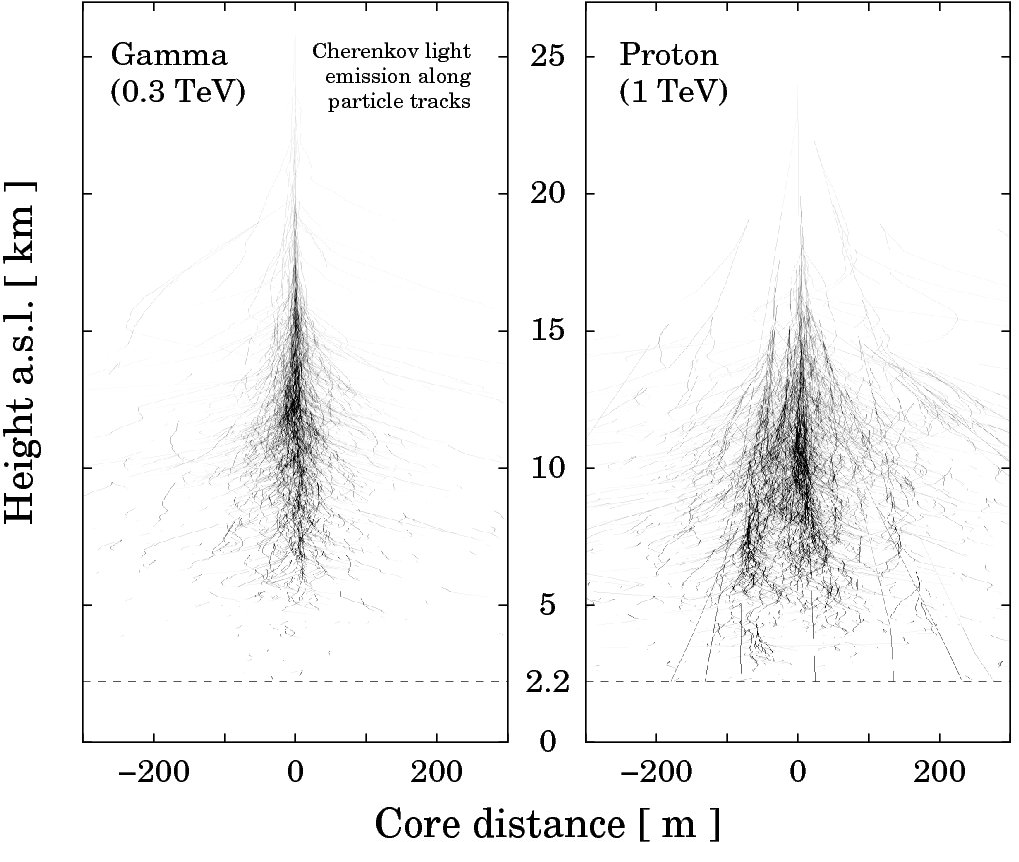
\includegraphics[width=0.95\textwidth]{images/showers_gamma_proton}
  \caption[Gamma Ray and Proton Showers]{
    A gamma ray shower alongside a proton shower.\cite{Bernlohr2008149}
  }
  \label{fig:gamma_vs_proton_airshower}
\end{figure}


\section{Galactic Center}
The galactic center is a complex region of space, with many astrophysical sources of gamma rays.
A disk of dust lies along the galactic plane, acting as an interaction medium for diffuse proton cosmic rays.
Nearby supernova remnants also produce gamma-rays as their expanding shell interacts with ambient dust.
The immediate area surrounding the galactic center a point-source emitter of gamma rays, though this mechanism is uncertain.

% black hole
Through kinematic observations of nearby stars, the galactic center has a supermassive black hole, with a mass of \SI{4e6}{\Msol} \cite{sgra_massdist}.
The Galactic Center also is a source of \TeV{} gamma rays, though the mechanism that produces them is still under debate.
% http://adsabs.harvard.edu/cgi-bin/bib_query?arXiv:1511.01159
One possibility is that the supermassive black hole emits particles, which convert into TeV gamma rays, while the second possibility suggests a nearby Pulsar Wind Nebula may be providing the gamma-ray-parent particles.
While the Galactic Center emits gamma rays, this emission is point-like to ground-based gamma ray telescopes. {\color{red}(rewrite this!??)}
This analysis instead focuses on the gamma ray flux outside this point-like inner angular region. {\color{red}(citation!??)}

The disk of gas present in the galactic plane acts as an interaction medium for passing cosmic rays, both from nearby galactic accelerators and from extragalactic sources.
These high-energy protons collide with the dust, shattering into $\pi^{\pm,0}$.
The $\pi^0$ then decays into two gamma rays {\color{red}??}, providing the diffuse emission.
The spectrum of this emission is {\color{red}??}.

% TeV gamma ray emission
% HESS
HESS sees excess around galactic center.


